% Added link to preamble
\documentclass[12pt]{article}
\usepackage[utf8]{inputenc}
\usepackage{blindtext}
\usepackage{graphicx}
\usepackage{tabularx}
\usepackage{authblk}
%\usepackage{natbib}
\usepackage{xcolor}
\usepackage{float}
\usepackage{amsmath}
\usepackage[english]{babel}
\usepackage{graphicx} % Required for inserting images
\usepackage[paperheight=16cm,paperwidth=12cm,textwidth=8cm]{geometry}
\usepackage[flushleft]{threeparttable,booktabs}

\usepackage[
        backend=biber,
        style=authoryear-comp,
        sorting=nyt,
        style=apa
    ]{biblatex}
 \addbibresource{references.bib}


 \geometry{
 a4paper,
 total={170mm,257mm},
 left=30mm,
 right=30mm,
 top=30mm,
 bottom=30mm
 }

% Keywords command
\providecommand{\keywords}[1]
{
  \small	
  \textbf{\textit{Keywords---}} #1
}

\graphicspath{{plot/}}



\addbibresource{}


\title{Names diffusion and social class}
\author{}
\date{May 2023}

\begin{document}

\maketitle

\section{Introduction}


\bigskip

\section{Theory}

\subsection{Culture and network analysis}

A very relevant approach to the study of inequalities is the analysis of social networks. This perspective of analysis has its origin in the works of Simmel 
 \parencite*{simmel_sociology_1964}, Blau \parencite*{blau_exchange_1986}, and White \parencite*{white_chains_1969,white_identity_2008}. Lomnitz's \parencite*{lomnitz_como_1975} work has been highly influential in Latin America. Following Harrison White's \parencite*{white_identity_2008} quote, social networks are informal and temporary organizational patterns that arise from uncertainty and control attempts by individuals and groups. In his perspective, the phenomenological reality of a network is "stories" and "identities," that is, traces of meaning from previous interactions encapsulated in stories that link identities. In this sense, any analysis of a structural nature that rules out the role of symbolic forms is reductionist and simplifying. Unlike Schutz, White is not interested in subjective meaning but in the substances that circulate in communication processes: in the stories that are told and in the identities that are constructed in those stories. Indeed, White's perspective forces us to glimpse mechanisms that describe the deployment of symbolic forms in creating identity limits. 
\bigskip

 It is frequently indicated that networks arise from individual success and failure, as well as from the development and emergence of medium- or large-scale social phenomena (inequalities, social movements, markets, academic fields, or political mechanisms) \parencite{blau_macrosociological_1977, gould_origins_2002, granovetter_strength_1973,lin_social_2002,mayhew_structuralism_1980}. In this sense, critical analytical elements have been identified to explain why inequality and social immobility go hand in hand \parencite{tilly_durable_2009} or why the redistribution of wealth affects only the symptoms of inequality, not its causes \parencite{diprete_relevance_2021}. For its part, work on social capital makes it easier to visualize the political need to enrich people's social networks (social capital) to provide opportunities that their interaction patterns do not offer \parencite{jackson_inequalitys_2021, lin_social_2002}.
\bigskip

As has often been suggested, network phenomena such as homophily and consolidation \parencite{dimaggio_how_2011, dimaggio_network_2012,jackson_inequalitys_2021,zhao_network_2021} tend to reinforce the initial resource endowments of certain social positions and the boundary categories that restrict intergroup exchange. Let's consider sociodemographic parameters that vertically differentiate a social space (for example, educational level). The logic is isomorphic \parencite{blau_macrosociological_1977}: the more socioeconomic inequality and the distance between level groups grow, the more the interaction rate. Between individuals with the same status marks \parencite{podolny_status_2008,smith_social_2014,torche_intergenerational_2014}. In the long run, this leads to the development and sedimentation of synergistic patterns of organizational segregation in broad sociodemographic spaces \parencite{mcpherson_blau_2004, tilly_durable_2009}. However, this approach has placed particular emphasis on the mechanisms that bias the diffusion patterns of "economic and material resources" to the detriment of other issues that flow through the networks, such as cultural traces (symbolic forms and styles), motivations individual and institutional \parencite{white_identity_2008}.
\bigskip

Structure and culture are not independent layers of the social \parencite{fuhse_dualities_2010,fuhse_theorizing_2015}. Social networks are spaces impregnated with cultural forms, at the same time that they are co-constructed. Thus, relationships are based on cultural models emulating (functional) institutions such as friendship or kinship, and the actors' identities are built in dynamic processes of attribution and negotiation within networks. In this sense, social categories and cultural models of relationships contribute to a particular ordering of the structure of social organization. Symbolic forms and styles \parencite{white_identity_2008} are disseminated and combined at the intersections of networks to promote the emergence of new styles and creativity.
\bigskip

White \parencite*{white_identity_2008} develops the concept of "catnet" to account for this duality. The fundamental idea is that networks are co-constituted with categories. In this sense, categories are linguistic representations that group similar actors to distinguish them from others. These categories-networks emerge as organizing elements from pre-existing categories that give a symbolic order to the actors of a sociodemographic space or from a densely connected population. Both sources are often reinforced. Categories usually occupy spaces and, together with other tendencies of social organization, such as homophily \footnote{Homophily is an ecological phenomenon and a fundamental organizing principle \parencite{blau_inequality_1977, mcpherson_birds_2001} and refers to the empirical tendency in which contact between similar people occurs at a higher rate than between different people. The omnipresence of homophily means that any information or resource that flows through the networks tends to be localized \parencite{small_enormous_2021}, one of the most relevant characteristics of the \parencite{mcpherson_baseline_2009, small_someone_2017, smith_social_2014}}, induce actors to relate to actors that make up the same category, reducing the chances of forming links between categories. Indeed, the categories act as triggers for social integration and disintegration. In highly unequal societies, local connectivity tends to predominate at the expense of global connectivity.
\bigskip

In this way, the categories are expected to be built as dense networks ("catnets") structurally and symbolically separated from other catnets \parencite{white_identity_2008}. This organizational process involves group closure dynamics that are generally symbolically and materially associated with developing social capital \parencite{burt_brokerage_2005} since it can facilitate the development of competitive advantages between groups that dispute access to resources. For example, closed networks involve people connected so their behavior does not go unnoticed, creating an advantage through reduced risk \parencite{burt_brokerage_2005}. Therefore, the ability to assess redundancy and density reduces control and transaction costs of valuable resources. Promoting, in this way, the location of resources and the exclusion of other groups.
\bigskip

A closed network provides ample bandwidth for the flow of stories as packets of personal data \parencite{burt_brokerage_2005}. The more closed the network, the more redundant the information accessible and the more widespread the detection. In this sense, detecting risks or bad behavior is the most relevant characteristic for developing trust in the flow and management of resources. However, the results of closure-type equity are mixed. Following the development of Burt \parencite*{burt_brokerage_2005} and Lin \parencite*{lin_social_2002}, "brokerage" is about coordinating people among whom it would be valuable but risky to trust, and "closure" is about making it safe to trust. Creating value is putting the two together and building closure around valuable bridging relationships. The closure is valuable when links between dense groups accompany it. Otherwise, exclusion processes are exalted and pernicious effects may arise in individual and group terms.
\bigskip

With this, it is reasonable to expect that favored groups will look for a closing build to control threats that can potentially jeopardize their positional advantage efficiently. Otherwise, their position of advantage makes it easier for them to occupy roles of management and coordination of valuable companies and interaction (e.g., exploitation) and access to disadvantaged social circles \parencite{erickson_culture_1996}. On the other hand, for underprivileged groups, the closure can help to consolidate their exclusion. In fact, following the argumentative line of social capital, combating poverty consists of increasing the possibilities of interaction with distant social circles and, eventually, consolidating bridges that facilitate interconnectivity and the flow of resources. In fact, in scenarios of high social inequality, mobility processes that involve upward interaction are unlikely. Hence the importance of studying them.

\subsection{Social and symbolic boundaries}

The categorical boundaries that groups construct and transmit are embedded in social networks with particular topologies. The population distribution and the diversity of sociodemographic groups determine these topologies. However, categorical boundaries contribute to the reproduction of these topologies and the distribution of resources and populations within them. In this sense, the categories are constituted by what Lamont conceptualizes as social and symbolic limits.
\bigskip

Social boundaries are the objectified forms of social differences manifesting in unequal access and unequal distribution of resources (material and immaterial) and social opportunities. They are also revealed in stable behavioral patterns of association, such as friendships, marriages, and membership in voluntary associations. Its functionality and its restrictive effect on the probabilities of interaction depend on the degree of agreement displayed that the symbolic limits reach. As Lamont indicates, they can only become social borders that operate as identifiable patterns of social exclusion or racial and class segregation \parencite{lamont_study_2002, tilly_social_2004, lamont_symbolic_2015}.
\bigskip

For their part, symbolic limits are conceptual distinctions that social actors make to categorize objects, people, practices, and even time and space. These distinctions can be expressed through normative interdictions, cultural attitudes and practices, and patterns of likes and dislikes. Symbolic boundaries also separate people into groups and generate feelings of similarity and belonging \parencite{lamont_symbolic_2015}.

They are tools by which individuals and groups struggle and agree on definitions of reality. At the same time, they are an essential means through which people gain status and monopolize resources \parencite{lamont_study_2002}. Indeed, symbolic borders play a crucial role in the creation of inequality and the exercise of power. Examining them allows us to capture the dynamic dimensions of social relations as groups compete in the production, dissemination, and institutionalization of alternative classification systems and principles.
\bigskip

For White \parencite*{white_identity_2008}, all interaction is driven by uncertainty. Because of this, individuals or groups (identities) try to establish "footing" (or consolidate a base) at the same time as establishing relative "control" in contexts. This is a basal organizational dynamic in which identities are constituted and resources diffused in social structures. Identities are defined in a communicative process through the stories they tell, and based on this, loyalties, prestige, and opinions are built, which contribute to consolidating identities' positions. Particularly relevant is that this communicative process involves cooperation and competition dynamics, and some identities may be more motivated to establish control and footing to protect access to resources.
\bigskip

White \parencite*{white_identity_2008} indicates that "styles" are an important cultural characteristic of network formations. Styles are evaluation parameters that allow individuals to perceive others as more or less similar. Thus, styles flow, adapt, and adopt based on mutual observation and emulation. From here, patterns of expression and communication emerge as collective experiences that contribute to developing identity borders and closure. The critical point is that dominant styles' influence does not depend on distance or direct interaction. Styles can circulate between social positions and even be exported from different cultures. Regarding networks, the effect of styles can occur in dyads or between structurally equivalent positions (i.e., with similar patterns of interaction).
\bigskip

In this perspective, identities are constructed as affiliations to multiple categories, circles, or social groups. The movement of identities between these limits contributes to the access and consumption of diverse cultural forms, and with this, individuals are shaping their own identities and stories. As identities involve locations, each person has their style, recognizable as a similarity of behavior in different situations \parencite{watts_identity_2002}.
\bigskip

As we indicated earlier, social categories are symbolic constructions that operate as boundaries restricting interaction between social groups. In short, they allow groups to "hoard opportunities" and "lockout" resources to outsiders \parencite{tilly_durable_2009}, resulting in a segregated network pattern with relatively small, densely connected groups separated from one another by symbolic limits and structural divisions, like the ordering suggested by the "catnet" concept or the "small world" metaphor \parencite{watts_collective_1998}. Thus, when intertwined with stories about the nature and differences of groups, the category becomes a self-fulfilling prophecy: it operates as a reading lens and as an executing agent of internal solidarity and rivalry between groups \parencite{fuhse_theorizing_2015}.

\subsection{Diversity, groups and cultural diffusion}

As indicated above, homophily can lead to the formation of distinct cultural groups. However, similar homophily can also lead to cultural homogeneity as groups become more like each other over time. Two main mechanisms can lead to cultural homogeneity: choice homophily and social influence \parencite{centola_homophily_2007}. Choice homophily refers to the tendency of similar people to associate with others who are similar to them. In contrast, social influence refers to the movement of people to become more like the people they associate with.
\bigskip

When choice homophily and social influence are present, they can lead to a process of local convergence, in which groups become more similar to one another. However, if there is enough heterogeneity in the population, this local convergence can also lead to global polarization, in which different groups become increasingly distant from each other \parencite{axelrod_dissemination_1997}. Added to the heterogeneity argument is growing social inequality, which differentiates a population in vertical terms. When heterogeneity tends to correlate with social inequality, categorical boundaries become more intense, and, indeed, interaction, resource flow, and social influence processes between polarized groups are less likely.
\bigskip

In this way, although homophily tends to homogenize groups over time, this tendency can establish categorical limits that are difficult to overcome in high inequality and growing heterogeneity. This can lead to a situation where cultural groups are so different that their members cannot interact beyond the group boundaries. This is not only a problem for the groups themselves but can also have negative consequences for society as a whole \parencite{centola_homophily_2007}. The key to these homophily dynamics is the changing nature of social interaction patterns \parencite{feld_describing_2007, centola_spontaneous_2015}. Changes in network topologies are facilitated by cultural influence and social adaptation processes, which allow individuals to evolve in the space of cultural ideas and behaviors. Indeed, by reducing similarity and interaction, links disappear, and new ones appear \parencite{feld_describing_2007, centola_homophily_2007}. This individual differentiation process eventually creates group consolidation since detachment from dissimilar people also gives rise to more robust bonds with similar individuals. This may be aggravated given the uncertainties that people who engage in upward or downward social mobility face. Following White (2008), jogging in these processes of changes in interaction patterns can be accompanied by even more marked homophily dynamics \parencite{blau_exchange_1986, white_identity_2008}.
\bigskip

Even though recent technological changes contribute to the development of greater diversity and, eventually, a more significant interaction between culturally diverse groups, the closing dynamics promoted by homophily and influence restrict our opportunities for affiliation or movement between communities and, thus, people with whom we choose to interact, share ideas, and adopt our patterns of life \parencite{mcpherson_birds_2001,mcpherson_blau_2004}. These patterns of preferential interaction of the similar produce cultural pockets whose identity and ideas, although flexible, have been stable since dissolution in a homogeneous global culture. While trends toward globalization provide more means of contact among more people, these same venues for interaction also show a strong tendency for people to self-organize into culturally defined groups, which may help preserve overall diversity \parencite{centola_homophily_2007}.
\bigskip
 
For this particular work, it is relevant to understand the dynamics of influence and social closure facilitated by homophily since people are more likely to adopt a behavior if they see that their close ones adopt it. Indeed, the probability of adopting a behavior decreases as the sociodemographic distance between an individual and those close to him increases, and the number of different behaviors in a network of close ones increases. Put like this, the social process of organizational segregation and the diffusion of behaviors, norms, and histories that distinguish and consolidate social categories among the groups of a sociodemographic space is determined in scope by the mechanisms of influence and homophily.
\bigskip

Contagion models of cultural transmission often assume that people only learn culture through meaningful and enduring relationships \parencite{goldberg_beyond_2018}. However, growing evidence suggests that cultural information can also be transmitted through surface interactions. Since all cultural exchange is an exchange of symbolic representations, cultural information can be transmitted rapidly. This means that cultural knowledge can be shared through brief interactions, such as observing someone's behavior or listening to them talk about their beliefs. Another reason that cultural information can be transmitted through surface interaction is that humans are innately attuned to the informative and normative behavioral cues of others. This means that we are naturally inclined to imitate the behaviors of others, even if we are not in a close relationship with them. Furthermore, the nature of the interpersonal relationship through which a cultural practice is observed becomes determinative for adoption only when the conduct involves significant risk. In such cases, observers are more likely to be influenced by peers they know and trust. 
\bigskip

On the other hand, it is plausible to think that when potentially imitable behaviors are associated with gains in terms of status, sociodemographic distance and the lack of significant ties are not restrictions to adopt such behaviors. Even over time, these behaviors can be adopted in waves and reinforced through diffusion and homophily. Content and meaning are essential for cultural diffusion. Adopting a cultural practice is an implicit consequence of the cultural meaning signaled to others through its adoption.

\subsection{Cultural tastes and class distinction}

\section{Methodology}

In this study, we used two data sources. The first corresponds to the number of names by year and commune from 1920 to 2022. These data were compiled by the Chilean civil registry and ceded for use in this study. Additionally, we work with census data from Chile. The goal of using this data is to build attributes of the names. Specifically, we assign weights based on the number of occurrences of the names by commune and year, which describe the (relative) socioeconomic conditions of the names. We use various social network analysis techniques, either for the descriptive or inferential analysis of the data. The methods used are described below:
\bigskip

\begin{enumerate}
  \item Descriptives: The descriptors are developed in two phases: first, we describe the data in its original state, that is, considering general distributions, for example, the number of new names per year within and between groups. Additionally, we look for patterns of stratification and segregation using the socioeconomic ranking imputed to each name. The latter can vary by year.
\bigskip

\begin{figure}[H]
    \centering
    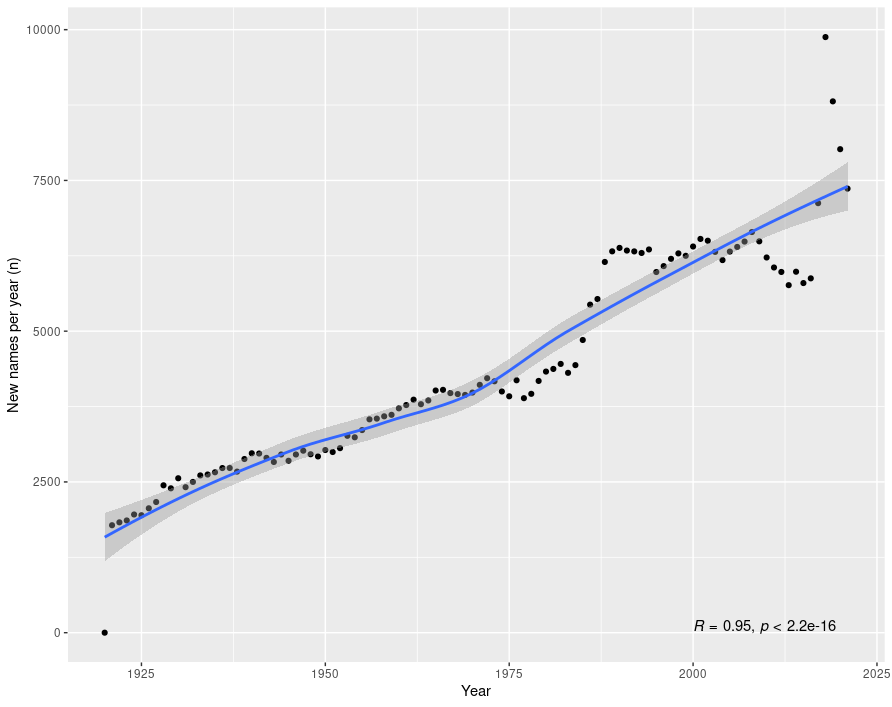
\includegraphics[width=13cm]{plot/new_names_yearII.png}
    \caption{Number of new names per year in Chile (1920-2022)}
    \label{}
\end{figure}

The previous graph considers all the data in a year, name, and commune format. The logic behind its construction is as follows: 1) we first get the unique names for each year (current year) and the previous year and get the difference. The results illustrate sustained growth with an average of 4380,088 new names per year and an average difference between years of 72.91.
\bigskip

Specifically, we construct an average annual socioeconomic level per commune. This was done by first calculating the average per household of Years of Education and Occupational Prestige, considering single-parent and two-parent households. After this, we calculate the annual median for the commune. These data were used to construct a socioeconomic index of the names, calculated considering the affiliation dyads per year of each name to each commune where it appears. Based on this structure, an average was calculated, weighted by the times the name appears in each commune by year. In this way, the index varies by year for each name. For the communes, there is variation considering only 6 sections in time that represent the population censuses of Chile (1960, 1970, 1982, 1992, 2002, 2017). Below, we can see the distribution of the measures at the community level.

\begin{figure}[H]
    \centering
    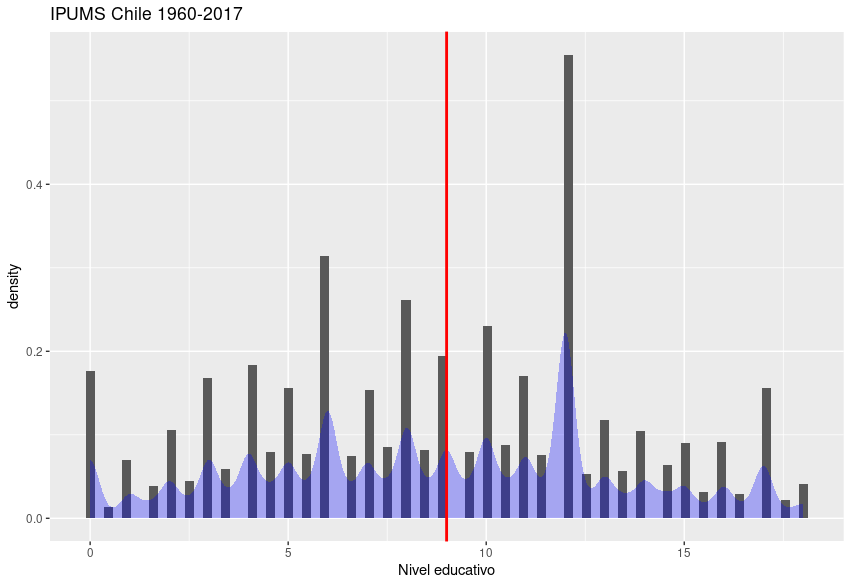
\includegraphics[width=13cm]{plot/nivel_educ.png}
    \caption{Distribution of educational years by commune for Chile  (1920-2022)}
    \label{}
\end{figure}



\begin{figure}[H]
    \centering
    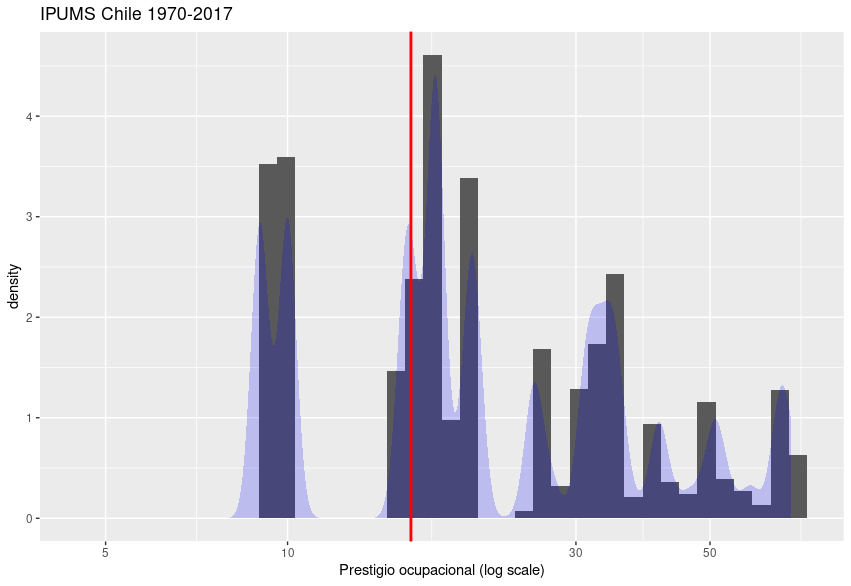
\includegraphics[width=13cm]{plot/occup_prestige.png}
    \caption{Distribution of occupational prestige by commune for Chile (1920-2022)}
    \label{}
\end{figure}


Additionally, we constructed annual socioeconomic quartiles for the names. This results in sequences of states from 1960 to 2021. With this data, we can visualize and analyze the flows of names between "socioeconomic levels" and patterns in the sequences (for example, using typical clustering techniques to analyze sequences). Below, we illustrate how names move between quartiles 4 and 1 over the years with flow maps.


\begin{figure}[H]
    \centering
    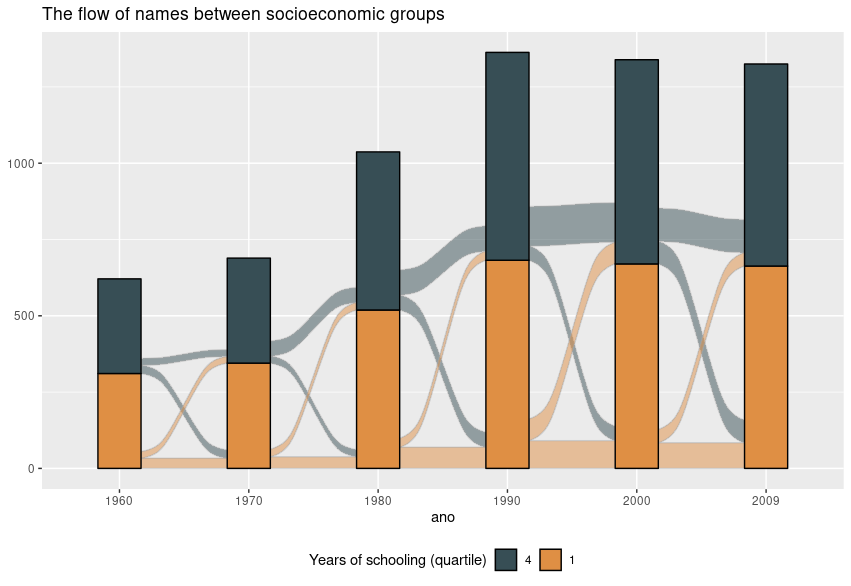
\includegraphics[width=13cm]{plot/flow_nivel_educ.png}
    \caption{The flow of names between educational groups}
    \label{}
\end{figure}


\begin{figure}[H]
    \centering
    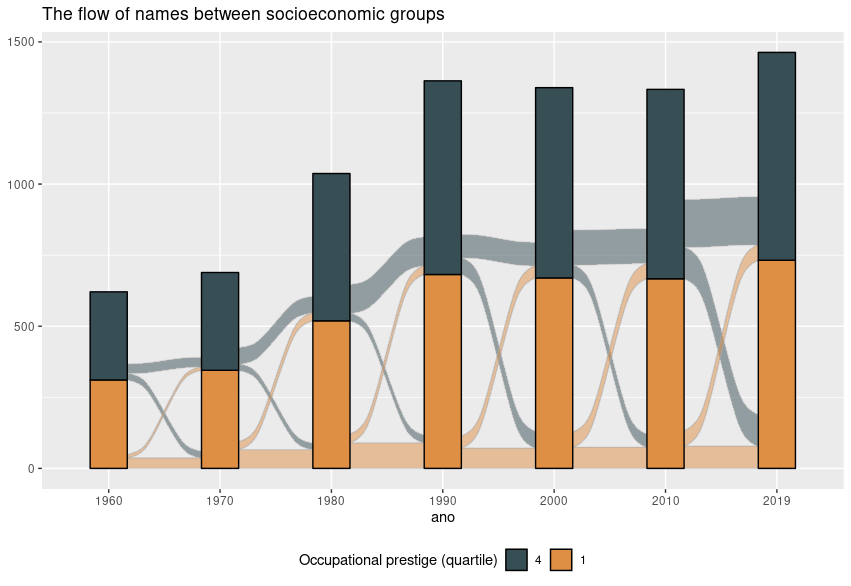
\includegraphics[width=13cm]{plot/flow_occup_prestige.png}
    \caption{The flow of names between occupational prestige groups}
    \label{}
\end{figure}



  \item Projection of valued bipartite matrices

Bipartite or two-mode networks (or multimodal networks) \parencite{knoke_multimodal_2021} involve two groups of entities and the relationships between them. Typically, the two-mode data structure involves relationships between entities, not within each entity type. When the data structure involves relationships "between" and "within" entities, this data structure is known as a \parencite{lazega_multilevel_2016} multilevel network. With our data, an entity can only connect to another of the same type using common links with the other kind of entity. For example, one way to think about the connectivity of an organizational field is through the multiple affiliations of actors \parencite{moody_structural_2003}.
\bigskip

Our original data includes two entities: 1) names and 2) communes. However, after performing a mode projection, we infer meaningful relationships between an entity type (names). It is worth indicating that when projecting one mode, we lose information: For example, if two individuals (mode 1) are connected to 3 organizations (mode 2), then they are connected in the projection by three links, and the weight of each link can be different. However, in the projection only one weight can be given.
\bigskip

We perform a weighted projection that implies that the obtained "mode one" network contains the minimum parallel of the observed interactions between two individuals of an entity. This means that if two individuals of one entity (A and B) interact with the same individuals of the other entity (a, b, c, d, e), for each of these links of entities A and B, it holds the minimum parallel value. For example, if the link A - b value is five and link B - b is 3, the kept value is 3. After this, the five minimum values are added to obtain the final weight of the link. The idea is that the similarity between A and B is due to their lower similarity in the interactions. We use the "bipartite" package designed for the R environment \parencite{dormann_bipartite_2022}.
\bigskip

  \item Bakcbone 

The previously obtained network in a weighted (or valued) way can be represented with a \(W\) matrix. Where \(W_{ij} \) indicates the link length between nodes \(i\) and \(j \). In our case, we do not consider directionality, which implies that \(W_{ij} = W_{ji}\). With the \(W\) matrix, we infer statistically significant links "within" the entity using the procedure developed by Serrano et al. \parencite*{serrano_extracting_2009}. We keep links considering 99\% (alpha = 0.05) confidence (This retains links with weights that are more likely than random after multiple permutations).
\bigskip

Serrano's approach, the "disparity filter" involves comparing the weights of the links with their expected values under a null model that considers the local community of each node. We used the backbone package for R (v2.1.1; Neal, 2022) to extract the unweighted backbone of a weighted and undirected unipartite network \parencite{neal_comparing_2021,serrano_extracting_2009}.
 \bigskip
 

We build simple network statistics, which contribute to making a picture of the topology of the networks built per year (or groups of years). Specifically, we calculated the size, the number of observed links, density, diameter, number of isolates, centralization, local and global transitivity, average degree, the standard deviation of degree, and average PageRank \parencite{brin_anatomy_1998}. Additionally, we search for cluster numbers and calculate modularity following the "info map" procedure. This algorithm detects network clusters based on random walks. The intuition is that a random walker is more likely to wander through the same community than travel to a different one. The "info map" algorithm considers an infinite random walk, which tends to go around one community until it passes to another; this method seeks to balance the number of communities and the number of unique identifiers in each community so that the path of the random walker can be recorded in the most accurate way \parencite{rosvall_maps_2008}. 
  
A continuadción mostramos los resultados de las redes construidas para todas las décadas, considerando una muestra del 10 \% de los datos completos. 
 \bigskip


\begin{sidewaystable}
    \centering
    \caption{Networks descriptives by decade}
      \small
  \renewcommand{\arraystretch}{1.2}
  \renewcommand{\tabcolsep}{0.1cm}
%\begin{tabular}{l*{10}{c}} 
\begin{tabular}{rrrrrrrrrrrrrr}
  \hline
 & size & edges & density & infomap\_n & modular & centraIg & g\_trans & l\_trans & DegreeAv & StdDegree & mpagerank & diameter & isolate \\ 
  \hline
1920-1929 & 60116.00 & 60116.00 & 0.33 & 120 & 0.01 & 1.66 & 0.41 & 0.91 & 199.72 & 248.15 & 0.00 & 3.00 & 603 \\ 
  1930-1939 & 89028.00 & 89028.00 & 0.38 & 145 & 0.00 & 1.61 & 0.44 & 0.90 & 260.70 & 300.57 & 0.00 & 3.00 & 684 \\ 
  1940-1949 & 107414.00 & 107414.00 & 0.45 & 164 & 0.00 & 1.55 & 0.48 &  & 309.55 & 326.12 & 0.00 & 3.00 & 695 \\ 
  1950-1959 & 131856.00 & 131856.00 & 0.51 & 180 & 0.00 & 1.48 & 0.53 & 0.89 & 367.80 & 353.96 & 0.00 & 2.00 & 718 \\ 
  1960-1969 & 174140.00 & 174140.00 & 0.61 & 221 & 0.00 & 1.39 & 0.58 & 0.88 & 458.87 & 396.06 & 0.00 & 2.00 & 760 \\ 
  1970-1979 & 187498.00 & 187498.00 & 0.64 & 227 & 0.00 & 1.35 & 0.60 &  & 488.91 & 405.77 & 0.00 & 3.00 & 768 \\ 
  1980-1989 & 250694.00 & 250694.00 & 0.78 & 273 & 0.00 & 1.21 & 0.65 &  & 623.62 & 447.55 & 0.00 & 3.00 & 805 \\ 
  1990-1999 & 324266.00 & 324266.00 & 0.81 & 318 & 0.00 & 1.17 & 0.65 &  & 726.24 & 501.94 & 0.00 & 3.00 & 894 \\ 
  2000-2009 & 324816.00 & 324816.00 & 0.81 & 310 & -0.00 & 1.18 & 0.63 &  & 723.42 & 506.09 & 0.00 & 3.00 & 899 \\ 
  2010-2019 & 327552.00 & 327552.00 & 0.91 & 317 & -0.00 & 1.08 & 0.65 &  & 769.80 & 487.78 & 0.00 & 3.00 & 852 \\ 
  2020-2022 & 42780.00 & 42780.00 & 0.76 & 113 & 0.00 & 1.20 & 0.63 & 0.87 & 254.64 & 184.42 & 0.00 & 3.00 & 337 \\ 
   \hline
\end{tabular}
\end{sidewaystable}

\bigskip




\item Bipartite Stochastic block models

Another analysis approach corresponds to the Stochastic Block Models for mode 2 networks. The Bipartite SBM models this network structure as a joint distribution of two adjacency matrices. These adjacency matrices are parameterized by a set of stochastic blocks, where each block represents the probability of connection between groups of nodes. The central idea of Bipartite SBM is that the likelihood of a connection between two nodes depends on the groups to which those nodes belong. Therefore, the model assumes that the links are not independent but are influenced by the nodes' membership in certain groups. The objective of the Bipartite SBM is to estimate the model's parameters, that is, the connection probabilities between the different groups of nodes, from the observed data of the bipartite network.

For illustrative purposes, we filter the complete data for all years (1920-2021) to consider the top 100 for all communes and adjust the scale of the tie intensity (or quantity). This way, I analyze a mode 2 network with 84 names and 38 communes, totaling 3071 dyads. The best-fitting model considers a structure of 5 blocks of communes and 4 blocks of names. The importance of Santiago and its communes concerning the rest is relevant. It seems that this line of analysis can also be carried out by decade, considering that there are extensions to do this with a longitudinal structure. In any case, we must do this considering a top of names and communes representing the flows.

Below, we illustrate with a graph:

\begin{figure}[H]
    \centering
    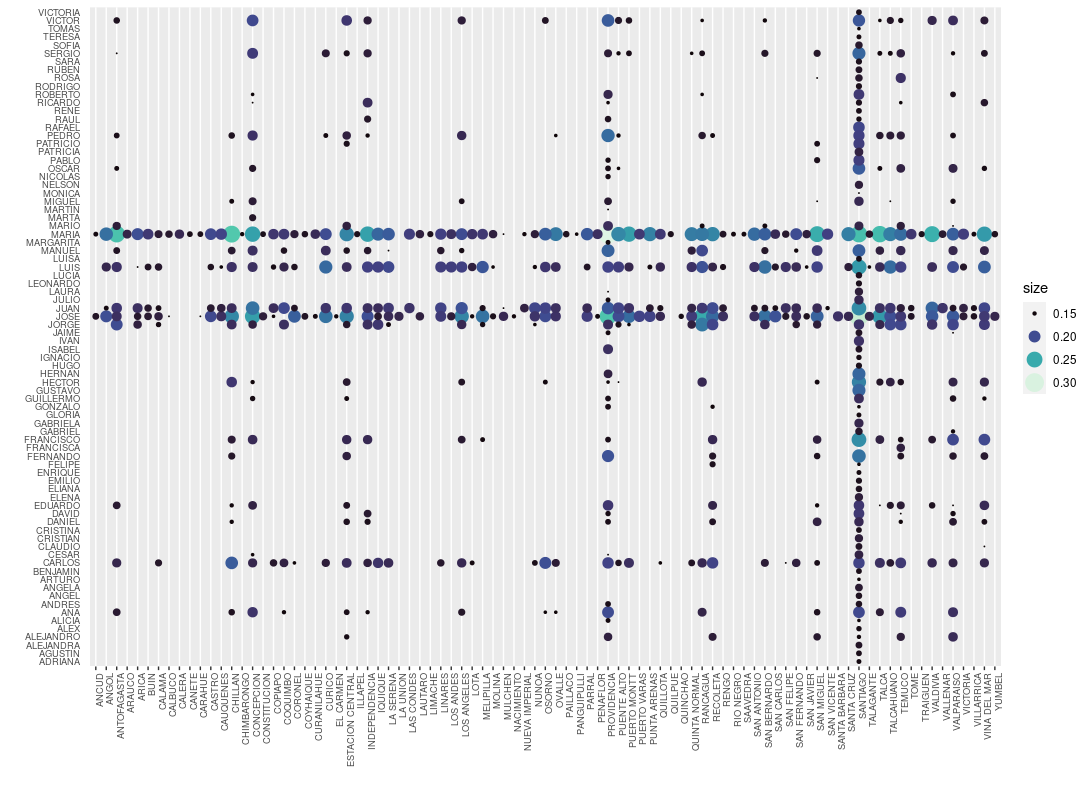
\includegraphics[width=13cm]{plot/name_commune.png}
    \caption{top names per commune in Chile (1920-2022)}
    \label{}
\end{figure}


\begin{figure}[H]
    \centering
    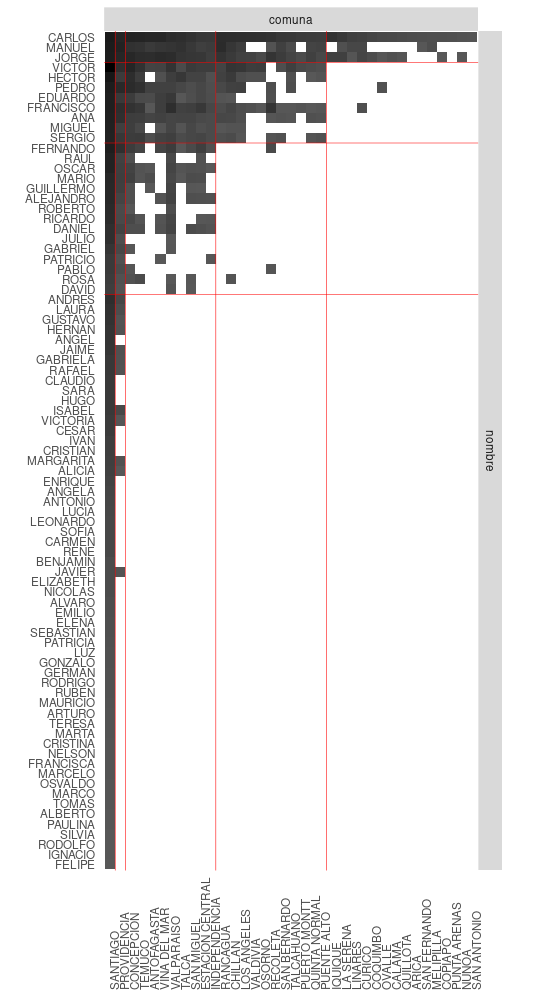
\includegraphics[width=10cm]{plot/blocks.png}
    \caption{Blocks top 100 names}
    \label{}
\end{figure}

\end{enumerate}

\section{Preguntas}

\begin{enumerate}
    \item Contagion: If we have an annual socioeconomic level for each name, we can ask ourselves how much of the average socioeconomic status of the names per year depends on the shared (average) socioeconomic level with other names. The shared status can be calculated by considering the strength of the communal co-presence of names i and j in a given period and the socioeconomic level of each name. This shared status would vary by name and year. Given the endogenous nature of this relationship, it must be instrumented, and this is a challenge since it implies constructing more variables for the names. In any case, the assumption would be that the linked attributes do not influence the socioeconomic level of the names but rather indirectly through the shared socioeconomic status or other characteristics of the names. 

    \item Dyadic analysis mode 1 (name-name): Here, we can model the strength of the intensity of the links between names. The questions could point towards analyzing the factors that influence the power of the ties. For example, it would be interesting to evaluate the effect of spatial proximity and the compositional effect (of communal contexts). Similarity and structural issues (such as triadic closure) would be the most influential factors for networks. 
    
\end{enumerate}


\section{Names diffusion}

En el trabajo de Bail, et al. \parencite*{bail_prestige_2019}, los autores recolectaron los 10 términos de búsqueda más populares y los 10 términos con mayor crecimiento en popularidad cada mes entre 2004 y 2014 para 199 países, usando datos de Google Trends (tendencias de búsqueda de Google). Esto resultó en una base de datos mensual que describe el comportamiento de búsqueda de individuos en 199 países durante este período. Para estudiar la difusión de términos de búsqueda entre países a través del tiempo, los autores construyeron un panel de datos con la siguiente structure:

\begin{enumerate}
\item La unidad de análisis es el par ordenado país A → país B en un año calendario determinado.
\item La variable de resultado es el recuento del número de términos de búsqueda que primero aparecieron en el conjunto de búsquedas más populares del país A y posteriormente en el país B dentro del mismo año calendario. Si un término apareció en A y luego en B en el mismo año, se contó como un caso de difusión en la dirección A→B.
\item El conjunto de datos resultante es un panel diádico-temporal con el país A, el país B, el año y el recuento de difusión como variables.
\end{enumerate}

Para emular la estrategia en el contexto Chileno usando datos de nombres entre comunas:

\begin{enumerate}
    \item La unidad de análisis sería el par ordenado comuna A → comuna B por cada año.
    \item La variable de resultado sería el conteo de nombres que primero aparecen en la comuna A y luego en la comuna B dentro del mismo año o el siguiente. Representando la difusión direccional de nombres.
    \item Las variables en el panel resultante serían la comuna A, la comuna B, el año y el conteo de difusión para cada par comunal por año.
\end{enumerate}

Para estudiar el fenómeno de la difusión de nombres entre comunas en Chile, construimos un conjunto de datos con estructura de panel dyádico que captura las relaciones direccionales en el tiempo entre pares de comunas. Específicamente, generamos todas las posibles diadas direccionales comuna A → comuna B para cada año entre 1920 y 2020, con A y B representando distintas comunas.
\bigskip

La variable de resultado en este conjunto de datos es el recuento anual de nombres que primero aparecen en una comuna A en un año dado, y posteriormente en una comuna B diferente dentro del siguiente año calendario. Este recuento indica entonces casos donde potencialmente ocurrió una difusión del uso de ciertos nombres desde residencias originales en una comuna, hacia residencias posteriores en nuevas comunas al siguiente año. Si bien no podemos confirmar que los nuevos casos del nombre en la comuna B se deban exclusivamente a un proceso de difusión desde A, la estructura direccional de los datos permite aproximar mediciones sobre tales patrones espacio-temporales de difusión de nombres entre comunas en Chile




\section{Nuevos descriptivos}


































\printbibliography

\end{document}
